\documentclass[12pt]{article}
\usepackage{amsmath,amssymb,mathrsfs}
\usepackage{graphicx,psfrag,color,float}
\usepackage[margin=1.8 in]{geometry}
\usepackage{titling,relsize,pifont}
\usepackage{algorithm}
\usepackage{grffile}
\usepackage{algpseudocode}
\usepackage{natbib}
\usepackage{url,enumerate}
\usepackage{setspace}
\doublespacing
\newtheorem{thm}{Theorem}
\newtheorem{lem}[thm]{Lemma}
\newtheorem{theorem}{Theorem}[section]
\newtheorem{assumption}{Assumption}
\newtheorem{lemma}[theorem]{Lemma}
\newtheorem{proposition}[theorem]{Proposition}
\newtheorem{corollary}[theorem]{Corollary}
\newenvironment{proof}[1][Proof]{\begin{trivlist}
\item[\hskip \labelsep {\bfseries #1}]}{\end{trivlist}}
\newenvironment{definition}[1][Definition]{\begin{trivlist}
\item[\hskip \labelsep {\bfseries #1}]}{\end{trivlist}}
\newenvironment{example}[1][Example]{\begin{trivlist}
\item[\hskip \labelsep {\bfseries #1}]}{\end{trivlist}}
\newenvironment{remark}[1][Remark]{\begin{trivlist}
\item[\hskip \labelsep {\bfseries #1}]}{\end{trivlist}}
%\pdfminorversion=4
% NOTE: To produce blinded version, replace "0" with "1" below.
\newcommand{\blind}{0}

% DON'T change margins - should be 1 inch all around.
\addtolength{\oddsidemargin}{-.5in}%
\addtolength{\evensidemargin}{-.5in}%
\addtolength{\textwidth}{1in}%
\addtolength{\textheight}{1.3in}%
\addtolength{\topmargin}{-.8in}%


\begin{document}

%\bibliographystyle{natbib}

\def\spacingset#1{\renewcommand{\baselinestretch}%
{#1}\small\normalsize} \spacingset{1}


%%%%%%%%%%%%%%%%%%%%%%%%%%%%%%%%%%%%%%%%%%%%%%%%%%%%%%%%%%%%%%%%%%%%%%%%%%%%%%

\if0\blind
{
  \title{\bf The Title}
  \author{$\mbox{Author1}^*$, Author2\thanks{Author1 is a graduate student and Author2 is Associate Professor, Department of Mathematics, Washington University in St. Louis, St. Louis, MO 63130.}
    \ and
    Author3 \thanks{Author3 is Professor, XXXXXX.}\\}
  \date{\vspace{-5ex}}
  \maketitle
} \fi

\if1\blind
{
  \bigskip
  \bigskip
  \bigskip
  \begin{center}
    {\LARGE\bf Title}
\end{center}
  \medskip
} \fi
\vspace{-3.5ex}
\begin{abstract}
blablablabla
\end{abstract}

\noindent%
\textbf{Key Words:} blablabla
%\vfill
\bigskip
\spacingset{1.40} % DON'T change the spacing!
\section{Introduction}
\label{sec:intro}

This is an introduction, blablabla.
%%%%%%%%%%%%%%%%%%%%%%%%%%%%%%%%%%%%%%%%%%%%%%%%%%%%%%%%%%
\section{Section 1}
\label{sec:sec1}
This is section 1.
%-------------------------------------------------------------------------------------------------% 
\section{Section 2}
\label{sec:sec2}
This is section 2.
%----------------------------------------------------
\subsection{subsec2.1}
This is subsection 2.1.

For linear model: \\
    We don't choose a subset of feature to run the regression, as the dataset is not such large. From the fitted vs residual plot we can find that it goes well at the beginning, but as fitted value getting bigger the residuals become not so well. But we can still think the residuals are equally spreaded around a horizontal line without distinct patterns, so there is no non-linear relationships.   \\
    
    \begin{figure}[h]
        \centering
        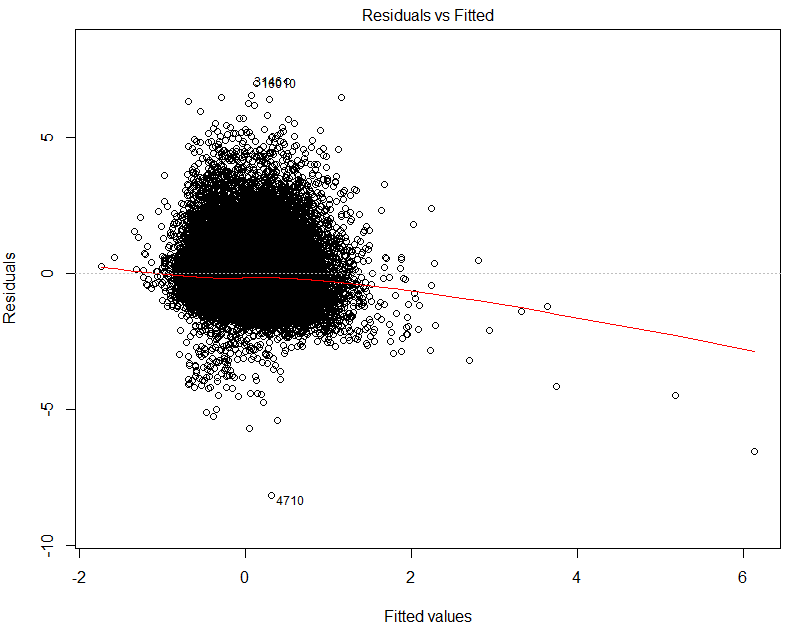
\includegraphics[width=\linewidth]{linear_fvsr.png}
        \caption{Linear Regression Plot: Fitted vs Residuals}
    \end{figure}  
    
    As we look QQ plot, it shows that the residuals are not normally distributed so well. So we should have a concern about the residuals distribuion.\\
    
    \begin{figure}[!]
        \centering
        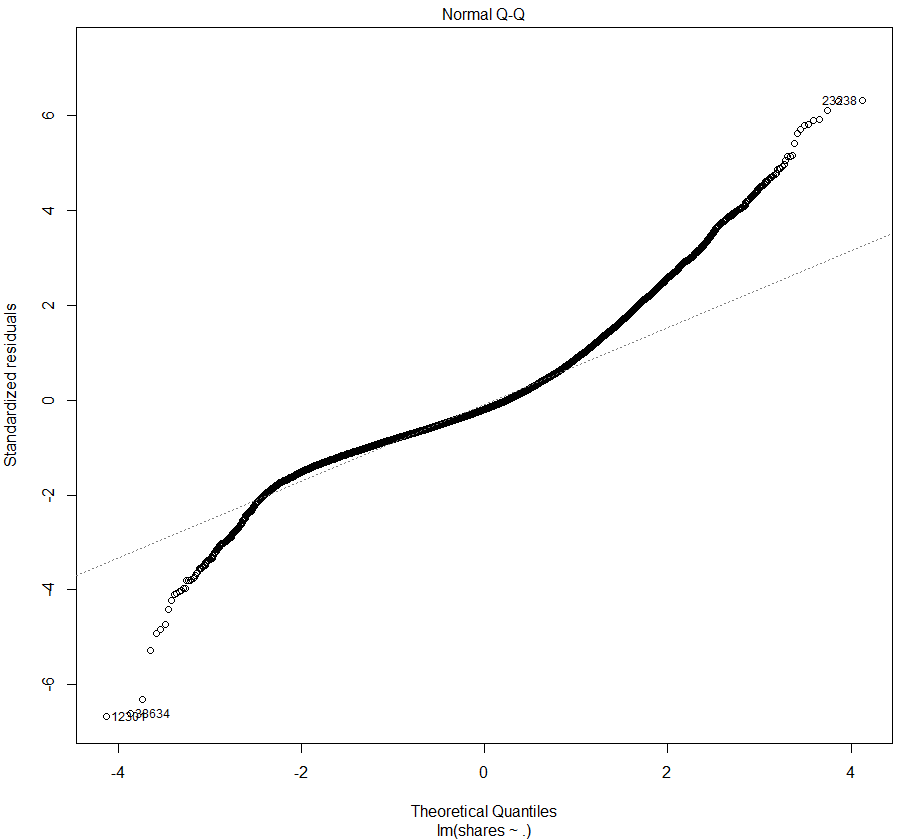
\includegraphics[width=\linewidth]{linear_qq.png}
        \caption{Linear Regression Plot: QQ plot}
    \end{figure}    
    From the Scale-location plot, we can see the red line is continually going up, which suggests that the assumptions of equal variance of the residuals may not be true.  \\
    \begin{figure}[!]
        \centering
        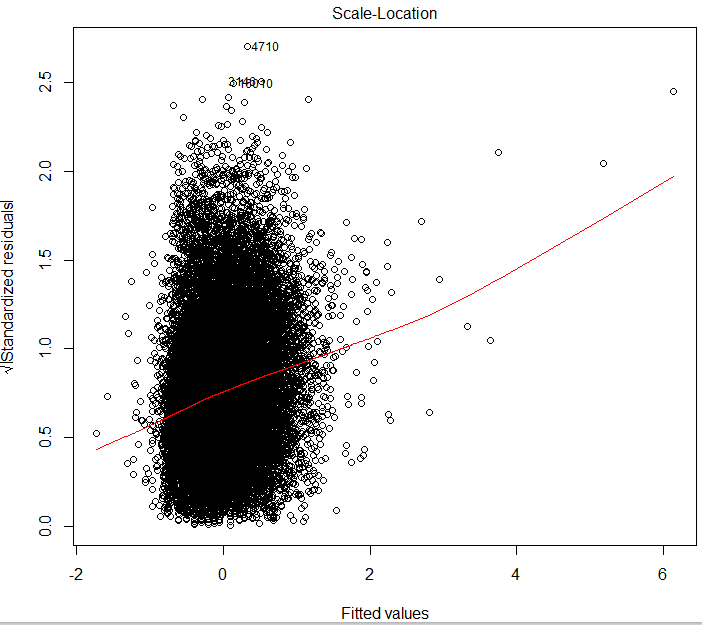
\includegraphics[width=\linewidth]{linear_sl.png}
        \caption{Linear Regression Plot: Scale-location}
    \end{figure}    
    For all variables, I calculate the vif for each of the variable, and some of their vif value are larger than 10, which shows the collinearity is significant in these variables. And we maybe can think about remove them. \\ 
For GAM: 
    From the method part, we know that $f_j(x_j)$ converges from $E \left[Y-\sum_{k \neq j}f_k(x_k)\mid{x_j} \right]$. We use gam model in R to fit the whole dataset, and according to model we get, we know that the number of local scoring iterations used to compute the estimates is only 9, which shows that this method converges pretty fast.

%-------------------------------------------------------------------------------------------------% 
\subsection{Subsec2.2}
This is subsection 2.2
%-------------------------------------------------------------------------------------------------% 
\section[Simulation Study]{Simulation results}\label{sec:sim}
This is the simulation part.
%-------------------------------------------------------------------------------------------------% 
\section{Discussion and conclusion}
\label{sec:conc}
The conclusion part.
%-------------------------------------------------------------------------------------------------% 
\setlength{\bibsep}{0pt plus 0.3ex}
\bibliographystyle{apalike}
{\footnotesize
\bibliography{myRef}  %create your own .bib file and cite them in the paper.
}
\end{document}
